% !TeX program = lualatex -synctex=1 -interaction=nonstopmode --shell-escape %.tex
\RequirePackage{luatex85,shellesc}

\documentclass[beamer,xcolor=dvipsnames]{standalone}
\RequirePackage[rus]{borochkin_tikz}

\begin{document}
\begin{standaloneframe}[shrink=0, fragile]
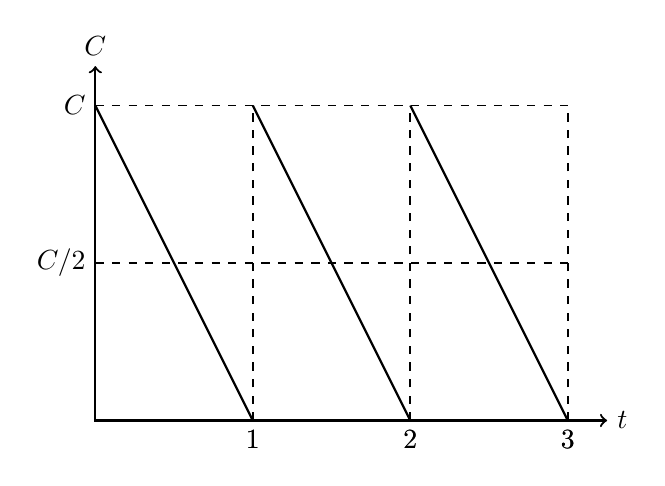
\begin{tikzpicture}
% grid 
%\draw[step=1cm,gray,very thin] (-1.9,-1.9) grid (5.9,5.9);
% axes
\draw [<->,thick] (0,4.5) node (yaxis) [above]{$C$}
|- (6.5,0) node (xaxis) [right] {$t$};

\draw[dashed](0,2)node[left]{$C/2$}--(6,2);

\draw[dashed](0,4)node[left]{$C$}--(6,4);

\coordinate(down) at (2,-4);
\coordinate(up) at (0,4);

\draw[thick](0,4)--++(down)node[below]{1}++(up)--++(down)node[below]{2}++(up)--++(down)node[below]{3}++(up);

\draw[thick,dashed](0,4)++(down)node[below]{1}--++(up)++(down)node[below]{2}--++(up)++(down)node[below]{3}--++(up);

\end{tikzpicture}

\end{standaloneframe}
\end{document}